\documentclass[10pt]{article}

\usepackage[margin=0.75in]{geometry}
\usepackage{amsmath,amsthm,amssymb}
\usepackage{xcolor}
\usepackage{cancel}
\usepackage{graphicx}
\usepackage{changepage}
\usepackage{circuitikz}
\usepackage{pgfplots}
\usepackage{physics}
\usepackage{hyperref}
\usepackage{minted}
\usepackage[breakable]{tcolorbox}
\usepackage[inline]{enumitem}

\theoremstyle{definition}
\newtheorem{problem}{Problem}
\newtheorem{soln}{Solution}

\pgfplotsset{compat=newest}
\usetikzlibrary{lindenmayersystems}
\usetikzlibrary{arrows}

\definecolor{incolor}{HTML}{303F9F}
\definecolor{outcolor}{HTML}{D84315}
\definecolor{cellborder}{HTML}{CFCFCF}
\definecolor{cellbackground}{HTML}{F7F7F7}
\newcommand{\eq}{=}
\tikzset
{%
  axes/.style={thick,-latex},
  cylinder/.style={right color=blue!80,left color=white,fill opacity=0.7},
  paraboloid back/.style={left color=magenta!80,fill opacity=0.4},
  paraboloid front/.style={left color=white, right color=magenta!80,fill opacity=0.4},
}

\makeatletter
\newcommand{\boxspacing}{\kern\kvtcb@left@rule\kern\kvtcb@boxsep}
\makeatother
\newcommand{\prompt}[4]{
    \ttfamily\llap{{\color{#2}[#3]:\hspace{3pt}#4}}\vspace{-\baselineskip}
}

\newcommand{\highlight}[1]{\colorbox{yellow}{$\displaystyle #1$}}

\newcommand{\volts}[0]{\mathrm{V}}
\newcommand{\amps}[0]{\mathrm{A}}
\newcommand{\ohms}[0]{\Omega}
\newcommand{\farad}[0]{\mathrm{F}}
\newcommand{\coulomb}[0]{\mathrm{C}}
\newcommand{\watts}[0]{\mathrm{W}}

\hypersetup{
    colorlinks=true,
    linkcolor=blue,
    filecolor=magenta,      
    urlcolor=cyan,
    pdftitle={Overleaf Example},
    pdfpagemode=FullScreen,
    }

\NewDocumentCommand{\evalat}{sO{\big}mm}{%
  \IfBooleanTF{#1}
   {\mleft. #3 \mright|_{#4}}
   {#3#2|_{#4}}%
}

\title{Physics 2130: Lab 1}
\author{Jeremy Favro}
\date{\today}

\begin{document}

\maketitle

% \begin{minted}[breaklines]{python}
% import matplotlib.pyplot as pyplot
% import numpy as np

% def plot_trimmed(path: str, label: str, mintime: float, minpos: float, maxtime: float) -> None:
%     data = np.loadtxt(path, delimiter=",", skiprows=1) # does this path syntax work on windows? who knows
%     data = data[ # not sure if there's a "smarter" way of doing this
%     (data[:, 0] > mintime) &
%     (data[:, 1] > minpos) &
%     (data[:, 0] < maxtime)
%     ]

%     times = data[:, 0]
%     positions = data[:, 1]
%     pyplot.figure(1)
%     pyplot.scatter(times, positions, label=label)
    
%     fit, cov = np.polyfit(times, positions, 2, cov=True)

%     # Without friction
%     fit_data = []
%     for t in times:
%         fit_data.append(fit[0]*t**2 + fit[1]*t + fit[2])

%     pyplot.plot(times, fit_data, label=label + "-fit", color="red")
%     pyplot.figlegend()
%     pyplot.xlabel("Time (s)")
%     pyplot.ylabel("Position (m)")
%     residual_data = []

%     for t in range(len(times)):
%         residual_data.append(fit_data[t] - positions[t])
%     pyplot.figure(2)
%     pyplot.plot(times, residual_data, label=label + "-residuals")
%     pyplot.figlegend()
%     pyplot.xlabel("Time (s)")
%     pyplot.ylabel("Position (m)")

%     # With friction - up
%     pyplot.figure(3)
%     max_val_index = np.argmax(positions)
%     positions_up = []
%     times_up = []
%     for i in range(0, max_val_index):
%         positions_up.append(positions[i])
%         times_up.append(times[i])

%     fit, cov = np.polyfit(times_up, positions_up, 2, cov=True)

%     up_fit_data = []
%     for t in times_up:
%         up_fit_data.append(fit[0]*t**2 + fit[1]*t + fit[2])

%     a_p = 2*fit[0]
%     a_p_u = np.sqrt(2*cov[0,0])
%     pyplot.plot(times_up, up_fit_data, label=label+"-friction-fit-up")
%     pyplot.plot(times_up, positions_up, label=label+"-friction-up")
%     pyplot.xlabel("Time (s)")
%     pyplot.ylabel("Position (m)")

%     # With friction - down
%     positions_down = []
%     times_down = []
%     for i in range(max_val_index - 1, len(positions)):
%         positions_down.append(positions[i])
%         times_down.append(times[i])

%     fit, cov = np.polyfit(times_down, positions_down, 2, cov=True)

%     down_fit_data = []
%     for t in times_down:
%         down_fit_data.append(fit[0]*t**2 + fit[1]*t + fit[2])
    
%     a_m = 2*fit[0]
%     a_m_u = np.sqrt(2*cov[0,0])
%     pyplot.plot(times_down, down_fit_data, label=label+"-friction-fit-down")
%     pyplot.plot(times_down, positions_down, label=label+"-friction-down")
%     pyplot.figlegend()
%     pyplot.xlabel("Time (s)")
%     pyplot.ylabel("Position (m)")
    
%     g = 9.8

%     print(f"{np.round(a_m, 2)}+-{np.round(a_m_u, 2)}")
%     print(f"{np.round(a_p, 2)}+-{np.round(a_p_u, 2)}")
%     theta = np.rad2deg(np.arcsin((a_m+a_p)/(-2*g)))
%     mu = (a_m-a_p)/(2*9.8*np.cos(theta))

%     print(theta)
%     print(mu)



% # plot_trimmed("./data/run1.csv", "run 1", .45, .1, 2.5)
% plot_trimmed("./data/run2.csv", "run 2", .5, .1, 2)
% # plot_trimmed("./data/run3.csv", "run 3", 1, .1, 3)
% pyplot.figlegend()
% pyplot.show()
% \end{minted}


\inputminted{python}{lab1c.py}
\newpage
This graph shows the recorded position-time data of the cart in blue and the result of polyfit in red.
The calculated acceleration is $\left(-1.888\pm0.001\right)ms^{-1}$ which is comparable to the acceleration found in part back
of $\left(-1.9\pm0.1\right)ms^{-1}$.
\\
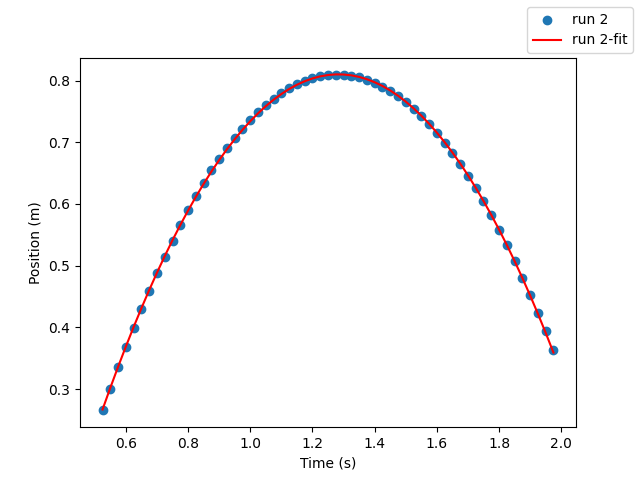
\includegraphics{Figure_1.png} \\ \newpage
This graph shows the residuals in the case where zero friction is assumed. The graph looks
non-random (though there is some randomness in the overall curve) and demonstrates that systematic error is a greater contributor to uncertainty than
random error.\\
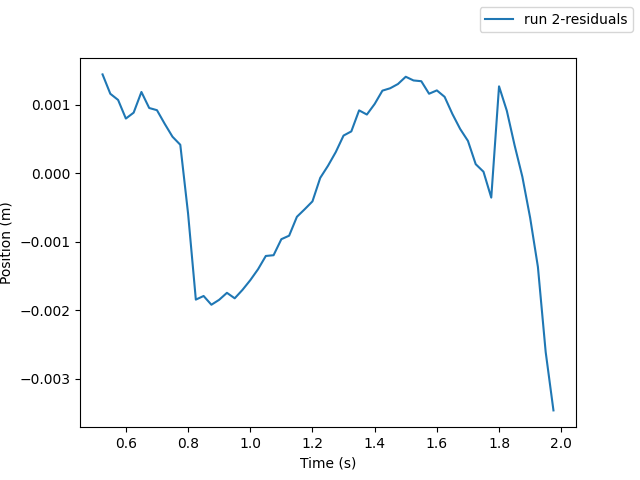
\includegraphics{Figure_2.png} \\ \newpage
This graph shows the position-time data split between travelling up the ramp and down the ramp, and the fits for each case.
The down/up $a_-=-1.852\pm0.003$ and $a_+=-1.923\pm0.004$ which make sense compared to the ``ideal''
acceleration found earlier as we'd expect $a_-<a$ as friction would slow it down and for the inverse reason we'd 
expect $a_+>a$ because friction is ``helping''. Using these acceleration values we can derive equations for $\mu$ and $\theta$
\begin{align*}
  & \mu=\displaystyle\frac{a_--a_+}{2g\cos\theta}=0.0334\\
  & \theta=\displaystyle\arcsin(\frac{a_-+a_+}{-2g})=11.104\deg 
\end{align*}
Both of which are reasonable as we don't expect friction to have an enormous impact given the difference between our ``real'' and ``ideal''
acceleration values is minimal and we expect the angle to be small as the acceleration parallel to the ramp is low compared to $g$.
\\
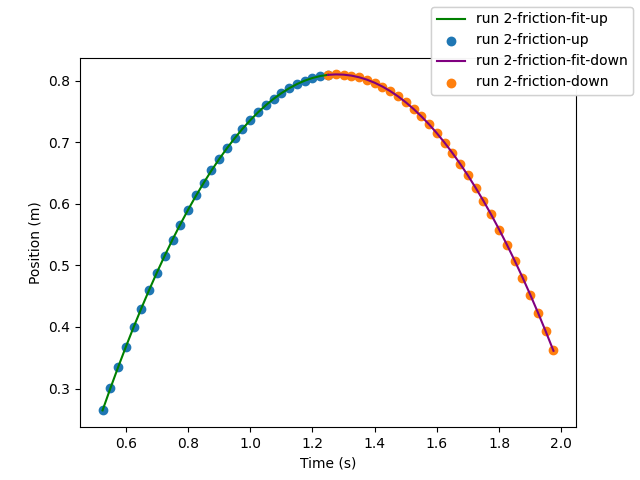
\includegraphics{Figure_3.png}\\

\end{document}